
From the previous investigation it is clear
that it is not possible to directly
incorporate the hydrogen energy
into the simulation.
The only key difference
between degenerate and
non-degenerate tunneling
however
is the location of the
electrons
immediately after
tunneling. Since
mixing only occurs
between states degenerate
in energy we expect
to see a lower energy
distribution in the
HCP site, however
in the
limit of a large
number of electrons
this energy
difference is negligible.
Since the off diagonal
interaction is small
we also find that the
individual electrons
transition at a much
faster rate than
hydrogen, and it is
reasonable
to expect that
the exact electron
distribution after a
transition has no effect
on the hydrogen dynamics.
This is the same reason that
we are able to assume separability
of the electron and hydrogen
density matrices in
\cref{sec:the redfield assumption}.
The electron distribution
during a transition however
should have an effect on the
rate, as an electron can
only transition to a state
which is previously
empty. The method used to
account for this behaviour
is discussed in
\cref{sec:corrected transition rate}.

\subsection{Rate at 150K}\label{sec:degenerate tunnelling simulaton}
To calculate the tunneling rate
we limit
ourselves to degenerate
hydrogen, making use of
the small band approach
discussed in \cref{sec:small band approach}
with a bandwidth set to target
tunneling in \(10^{-9}s\).
The hydrogen occupation
was seen to oscillate
rapidly inside a wavepacket
which was fitted to
\(\exp{(-{ (Rt)}^2)}\).

the occupation fraction
\(N = \frac{n}{s}\) was
varied by changing the
number of electrons (\(n\))
and number of states (\(s\)),
plotted in
\cref{fig:occupation rate curve}.
\begin{figure}
    \centering
    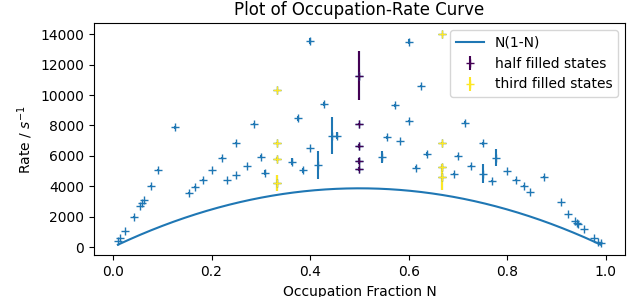
\includegraphics[width=0.7\linewidth]{Figures/Simulation/Occupation Rate Curve.png}
    \caption{Plot of the occupation-rate curve
        at 150K, with the predicted rate from half
        filled data. The rate is seen to
        tend to a constant
        value as the number of states
        \(s\rightarrow{}\infty{}\).
    }\label{fig:occupation rate curve}
\end{figure}
The rate is seen to change
at constant \(N\) as the
number of states is
increased however the asymptotic
behaviour appeared to follow the
simple form
\begin{equation}
    R(N,N) = 4 R_0 N(1-N)\label{eqn:degenerate tunnelling rate}
\end{equation}
where \(R_0\) is the
rate constant to be determined.
This is exactly the rate curve
we see in the Lindblad
analysis when hydrogen tunnelling
is paired with a single
electron transition.
Repeating the measurements at several
temperatures it was not possible
to identify any
temperature dependance of the
rate constant \(R_0\).

\subsection{Calculating \(R_0\)}\label{sec:calculating R0}
Since the rate depends only on a single
parameter \(R_0\) we are able to
extrapolate the rate from
the asymptotic
limit at a single
occupation fraction. This can
only be achieved for
\(N=\frac{1}{2}\), where
by far the largest number of
datapoints were collected (\cref{fig:half filled rate}).
\begin{figure}[htbp]
    \centering
    \begin{subfigure}{0.45\linewidth}
        \centering
        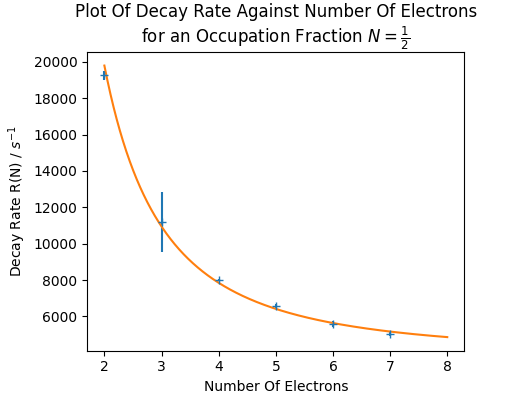
\includegraphics[width =0.9 \linewidth]{Figures/Simulation/Decay rate against electrons N=0.5.png}
        \caption{Half Filled Rates
        }\label{sub@fig:plot of half filled rates}
    \end{subfigure}
    \hfill
    \begin{subfigure}{0.45\linewidth}
        \centering
        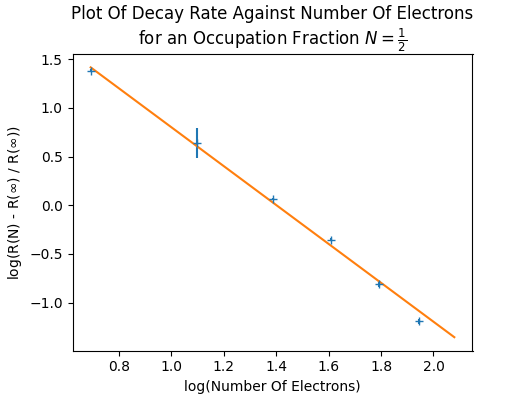
\includegraphics[width = 0.9\linewidth]{Figures/Simulation/Decay rate against electrons N=0.5 log.png}
        \caption{\(\log{}\) Half Filled Rates
        }\label{sub@fig:log plot of half fileld rates}
    \end{subfigure}
    \caption{Plot of the decay rates against
    number of electrons \(n\) for
    \(N=0.5\). The decay rates were
    fitted to
    \(R(n) = R(\infty) + {(\frac{A}{n})}^2\)
    where \(R(\infty) = R_0\) was
    found to be \(3900\pm 100s^{-1}\).
    }\label{fig:half filled rate}
\end{figure}
We are also able to extrapolate
\(R_0\) from the asymptotic
rates for states with n electrons.
As \(N\rightarrow{}0\)
we find
\(R(N,N) \sim{} 4 R_0 N = 4R_0 (\frac{n}{s})\).
We are therefore able to
use the gradient as the
number of states \(s\rightarrow{}\infty{}\)
to find \(R_0\).
Since the rate curve
is symmetric we expect
identical behaviour for
n holes, however
since the 1 electron
data was inconsistent (\cref{sub@fig:one electron rates})
we limit the analysis to 2 electron
or 2 hole data.
\begin{figure}[htbp]
    \centering
    \begin{subfigure}{0.45\linewidth}
        \centering
        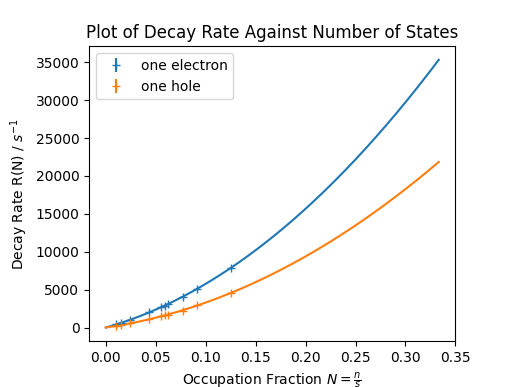
\includegraphics[width =0.9 \linewidth]{Figures/Simulation/Decay rate against occupation n=1.png}
        \caption{1 Electron Data
        }\label{sub@fig:one electron rates}
    \end{subfigure}
    \hfill
    \begin{subfigure}{0.45\linewidth}
        \centering
        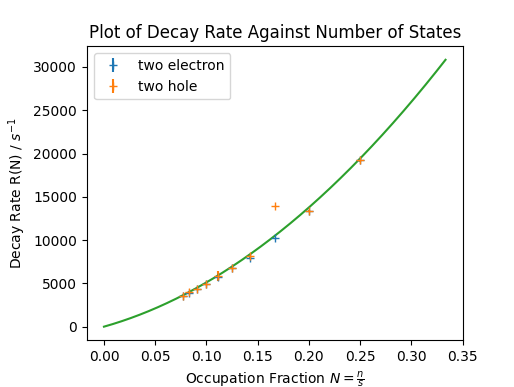
\includegraphics[width = 0.9\linewidth]{Figures/Simulation/Decay rate against occupation n=2.png}
        \caption{2 Electron Data
        }\label{sub@fig:two electron rates}
    \end{subfigure}
    \caption{Plot of the asymptotic
        form of the decay rates as \(N\rightarrow{}0\)
        at a fixed number of electrons \(n\).
        The single electron and single
        hole data is inconsistent
        (\cref{sub@fig:one electron rates}),
        however the two electron data
        was fitted to \(R(N) = 4R_0N + AN^2\)
        to give an overall rate constant
        \(R_0 = 8400\pm 600s^{-1}\). This is
        unlikely to give an accurate
        representation of the
        true decay rate, as it predicts
        a rate at \(N=0.5\)
        well above that measured even
        for \(n=5\) electrons.
    }\label{fig:small N rate}
\end{figure}
The \(N=\frac{1}{2}\) data
gave a rate constant
\(R_0 = 3900\pm 100s^{-1}\),
and for the \(n=2\) data
we find \(R_0 = 8400\pm 600s^{-1}\).
The decay rate suggested
from the \(N=2\) data is
unlikely to give an accurate
representation of the
decay rate, as it predicts
an asymptotic rate at \(N=0.5\)
well above that measured even
for \(n=5\) electrons.

\subsection{Corrected Transition Rate}\label{sec:corrected transition rate}
In the real hydrogen
system energy is conserved
during tunneling,
which leads
to the electron loosing energy
as the hydrogen transitions from
FCC to HCP sites
(\cref{sec:different hydrogen energy}).
To correct for this behaviour
we need to find the tunneling
rate from an occupation \(N\)
to an occupation \(N'\).
Due to
the arguments outlined in
\cref{app:combined tunnelling rates}
a general system with a different
forward and backward rate the
combined tunneling rate is
given by
\begin{equation}
    R(N,N') = R(N\rightarrow{}N') + R(N'\rightarrow{}N)
\end{equation}
where \(R(N\rightarrow{}N')\), \(R(N'\rightarrow{}N)\)
are the forward and backwards
tunneling rates respectively.
There are
three obvious ways to modify the tunneling
rate
\begin{align}
    R(N\rightarrow{}N') & = 2R_0N(1-N)           \label{eqn:no correction rate}     \\
    R(N\rightarrow{}N') & = 2R_0N(1-N')          \label{eqn:target correction rate}
\end{align}
all of which have the correct
limit in the case \(N=N'\),
when the forward rate is half
of the total rate given
by \cref{eqn:degenerate tunnelling rate}
\begin{equation}
    R(N\rightarrow{}N) = 2R_0N(1-N)
\end{equation}
The interpretation of these
corrections are
simple. \cref{eqn:no correction rate}
assumes the rate only depends
on the initial occupation and
\cref{eqn:target correction rate} assumes the rate
depends on the probability the
initial state is occupied
\(N\) and the final state
is unoccupied \(1-N'\). We could
also consider a correction
\begin{equation}
    R(N\rightarrow{}N') = 2R_0 \sqrt{N(1-N)N'(1-N')} \label{eqn:two hop correction}
\end{equation}
which implies a two jump process.
The electron falls to a lower band
before being promoted back into
its original location, with
each jump contributing \(\sqrt{N(1-N')}\)
to the rate. Note we have ignored functions
such as \(2R_0N'(1-N')\) which
would give the same overall rate
as \(2R_0N(1-N)\).

\subsection{Total Tunnelling Rate}
To recover the total tunneling
rate the occupation rate curve
is converted into an
energy rate using the
fermi-dirac distribution.
For \(R(N\rightarrow{}N') = 2R_0N(1-N')\)
we find
\begin{align}
    N(\epsilon)                         & = \frac{1}{1 + \exp{(\beta(\epsilon - \mu))}}                                                                         \\
    R(\epsilon \rightarrow{} \epsilon') & = 2R_0 \frac{1}{1 + \exp{(\beta(\epsilon - \mu))}}(1- \frac{1}{1 + \exp{(\beta(\epsilon' - \mu))}})                   \\
                                        & = 2R_0 \frac{\exp{(\beta(\epsilon' - \mu))}}{(1 + \exp{(\beta(\epsilon - \mu))})(1 + \exp{(\beta(\epsilon' - \mu))})}
\end{align}
where we have assumed uniform
occupation within a band.
The rate curve
(\cref{fig:tunneling rate against energy})
can then be
integrated to give an
overall tunneling rate, the results of
which are given in \cref{tab:decay rates simulated 150K}.
\begin{figure}[htbp]
    \centering
    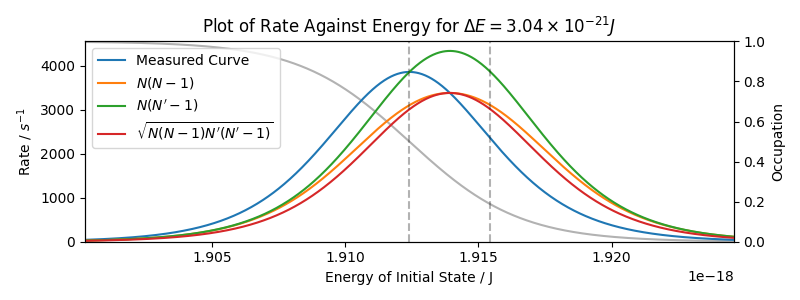
\includegraphics[width =0.9 \linewidth]{Figures/Simulation/Corrected Decay Rates.png}
    \caption{Plot of the corrected
        tunneling rate curve against
        energy. As the occupation curve
        (shown in grey) falls to 0
        the rate falls also. The corrected
        rate is seen to peak at half of the hydrogen
        energy difference above the fermi
        energy (grey dashed line).
    }\label{fig:tunneling rate against energy}
\end{figure}

\begin{table}[htbp]
    \begin{center}
        \begin{tabular}{ *{3}{c} }
            \toprule
            Rate                      & \(\frac{1}{2}\) Filled \(10^{9} s^{-1}\) & 2 Electron \(10^{9} s^{-1}\) \\
            \midrule
            Uncorrected               & \(3.6\pm 0.1\)                           & \(7.9\pm 0.6\)               \\
            \(N(1-N)\)                & \(3.6\pm 0.1\)                           & \(7.87\pm 0.6\)              \\
            \(N(1-N')\)               & \(4.3\pm 0.1\)                           & \(9.24\pm 0.7\)              \\
            \(\sqrt{N(1-N)N'(1-N')}\) & \(3.3\pm 0.1\)                           & \(7.20\pm 0.6\)              \\
            \bottomrule
        \end{tabular}
    \end{center}
    \caption{Comparison
    of decay rates at 150K.
    The tunneling rates
    taken from the
    \(\frac{1}{2}\) filled
    data is close to the
    experimental rate of
    \(3.3\times{}10^{9}s^{-1}\).
    As discussed in
    \cref{sec:calculating R0}
    the two electron decay
    represent a large
    overestimate of the
    true tunneling rate.
    }\label{tab:decay rates simulated 150K}
\end{table}

\subsection{Investigating Rate Corrections}
Given the calculated tunneling rates
it is possible to compare
the temperature dependence
with experiment.
As no temperature dependence
could be seen in the
simulation we use
the same rate constant calculated
at \(150K\) at all temperatures.
The temperature dependence
is therefore entirely
due to the corrections
made in
\cref{sec:corrected transition rate}.
The tunneling rates
plotted in
\cref{fig:simulation-experiment comparison}
show good agreement with
those measured in experiment.
\begin{figure}[htbp]
    \centering
    \begin{subfigure}{0.45\linewidth}
        \centering
        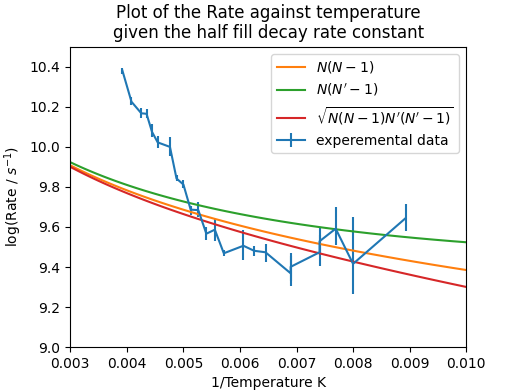
\includegraphics[width =0.9 \linewidth]{Figures/Simulation/Decay rate against temperature half fill 150K 1 spin.png}
        \caption{Half Filled Data
        }\label{sub@fig:half filled rates with experiment}
    \end{subfigure}
    \hfill
    \begin{subfigure}{0.45\linewidth}
        \centering
        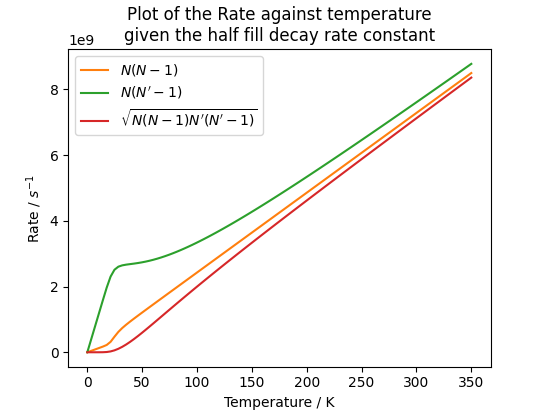
\includegraphics[width = 0.9\linewidth]{Figures/Simulation/Decay rate against temperature half fill 150K 1 spin low temp.png}
        \caption{Large Temperature Range
        }\label{sub@fig:simulation temperature dependence comparison}
    \end{subfigure}
    \caption{Plot of the decay rates
        against temperature with a comparison
        to experiment. The half
        filled data provided a good
        fit to the experimental
        tunneling rates
        (\cref{sub@fig:half filled rates with experiment}).
        The three methods of correcting
        the rate introduced in
        \cref{sec:corrected transition rate}
        gave a similar temperature
        dependence, all of which were consistent
        with experimental
        data. If we look at
        the high temperature
        limit
        \cref{sub@fig:simulation temperature dependence comparison}
        the tunneling
        rate is seen to converge
        as \(N\rightarrow{}N'\).
        The rates are seen to diverge
        at \(25K\) however this is well
        below the range of temperatures
        measured in experiment.
    }\label{fig:simulation-experiment comparison}
\end{figure}

Outside the experimentally
relevant range we see that the
tunneling rates remain
similar at all temperatures
(\cref{sub@fig:simulation temperature dependence comparison}).
Although we have no way
to predict the behaviour at
such low temperatures, the
choice \(\sqrt{N(1-N)N'(1-N')}\)
exhibits much smoother
behaviour as \(T\rightarrow{}0\).
With comparison to the lindblad
equation however
(\cref{sec:lindblad corrected tunneling})
the \(N(1-N')\)
correction seems to be the
most physically justifiable.



\subsection{Tunneling Without Self Interaction}\label{sec:tunnelling no diagonal}
In \cref{sec:different hydrogen energy}
it was found that the diagonal interaction
prevented mixing of the FCC and HCP
sites once hydrogen energy was introduced
to the experiment. It is therefore
useful to investigate the extent
to which this interaction
effects the interaction (\cref{fig:non diagonal decay rates}).
\begin{figure}[htbp]
    \centering
    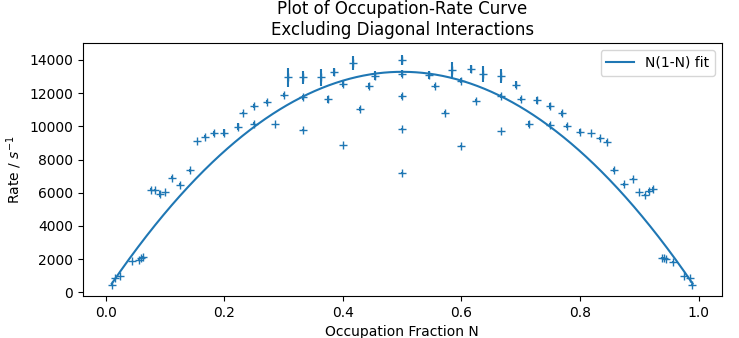
\includegraphics[width=0.7\linewidth]{Figures/Simulation/Occupation Rate Curve No Diagonal.png}
    \caption{Plot of decay rates measured without
        the inclusion of diagonal interaction.
        We see a much larger rate constant (\(R_0 \sim{} 13000 s^{-1}\)),
        and the rates are seen to
        increase (rather than
        decrease) as \(n\rightarrow{}\infty{}\).
    }\label{fig:non diagonal decay rates}
\end{figure}
The data gave
a rate constant
of \(R_0 \sim{} 13000 s^{-1}\),
more than \(3\times{}\) that seen in
the full interaction.
It is therefore
clear that this self interaction
has an important role
in the simulated
tunneling rate, and
removing such an interaction
is not a valid approach to
calculate a non-degenerate
tunneling rate.

\subsection{Simulation With Multiple Spins}



\subsection{Simulation With Multiple Hydrogen Sites}
In the real Nickel lattice the FCC and
HCP sites are arranged in a regular
lattice, such that there are \ldots
neighbouring HCP site of each FCC
hydrogen. In future investigations
it should be therefore be
possible to include the
effect of a larger number of
hydrogen sites,




\subsection{Bosons with Constrained Occupation}
To investigate the effect of fermion spin
statistics \ldots to calculate the rate
for bosons.
